
%----------------------------------------------------------------------------------------
%	PACKAGES AND OTHER DOCUMENT CONFIGURATIONS
%----------------------------------------------------------------------------------------



\documentclass[12pt]{article} % Default font size is 12pt, it can be changed here
\usepackage{cite}
\usepackage{url}
\usepackage{geometry} % Required to change the page size to A4
\geometry{a4paper} % Set the page size to be A4 as opposed to the default US Letter
\usepackage{graphicx} % Required for including pictures
\usepackage{float} % Allows putting an [H] in \begin{figure} to specify the exact location of the figure
\usepackage{wrapfig} % Allows in-line images such as the example fish picture
\linespread{1.2} % Line spacing
%\setlength\parindent{0pt} % Uncomment to remove all indentation from paragraphs
\graphicspath{{./Pictures/}} % Specifies the directory where pictures are stored
\usepackage{tabularx}



\usepackage{fancyhdr}
\pagestyle{fancyplain}
\fancyfoot[C]{Sander Martens}
\fancyfoot[R]{\thepage}


\begin{document}

%----------------------------------------------------------------------------------------
%	TITLE PAGE
%----------------------------------------------------------------------------------------

\begin{titlepage}

\newcommand{\HRule}{\rule{\linewidth}{0.5mm}} % Defines a new command for the horizontal lines, change thickness here

\center % Center everything on the page

\textsc{\LARGE Provinciale Hogeschool Limburg}\\[1.5cm] % Name of your university/college
\textsc{\Large Toegpaste informatica}\\[0.5cm] % Major heading such as course name
\textsc{\large Linux}\\[0.5cm] % Minor heading such as course title

\HRule \\[0.4cm]
{ \huge \bfseries Individuele opdracht}\\[0.4cm] % Title of your document
\HRule \\[1.5cm]

\begin{minipage}{0.4\textwidth}
\begin{flushleft} \large
\emph{Geschreven door:}\\
\textsc{Sander Martens} % Your name
\end{flushleft}
\end{minipage}
~
\begin{minipage}{0.4\textwidth}
\begin{flushright} \large
\emph{Leerkracht:} \\
 \textsc{Mnr. Willekens} % Supervisor's Name
\end{flushright}
\end{minipage}\\[4cm]

{\large \Today}\\[3cm] % Date, change the \today to a set date if you want to be precise

\vfill % Fill the rest of the page with whitespace

\end{titlepage}

%----------------------------------------------------------------------------------------
%	TABLE OF CONTENTS
%----------------------------------------------------------------------------------------

\tableofcontents % Include a table of contents

\newpage % Begins the essay on a new page instead of on the same page as the table of contents 

\listoffigures

\newpage % Begins the essay on a new page instead of on the same page as the table of contents 

\listoftables

\newpage % Begins the essay on a new page instead of on the same page as the table of contents 

%----------------------------------------------------------------------------------------
%	INTRODUCTION
%----------------------------------------------------------------------------------------

\section{Gnome-Do} % Major section



%------------------------------------------------
\subsection{De geschiedenis} % Sub-section
De man die aan de basis staat van Gnome-do is David Siegel. Alles begon aan de Universiteit van Pennsylvania. Siegel volgde computerwetenschap aan de universiteit van Pennsylvania waar hij voor zijn project het design document schreef. Tevens ontwierp hij de zoek- en plugin architectuur en startte een gratis software project op over het Gnome-Do. Alsof dat nog niet genoeg was, schreef Siegel ook de eerste plugin-set. Deze set bevatte Firefox, Evolution, bestanden, mappen, applicaties, Ryhtmbox, Pidgin, Epiphany en terminal plugins samen met andere fundementele plugin componenten. In 2008 studeerde Siegel af en probeerde alsnog andere studenten aan te moedigen om actief deel te nemen aan zijn project en zo de toekomst van Gnome-do meer vorm te geven. Gnome-do is gebaseerd op Quicksilver and GNOME Launch Box. De eerste release van Gnome-Do werd uitgebracht op 6 februari 2008. \cite{David}

\begin{figure}[H]
\center{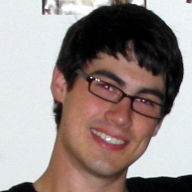
\includegraphics[width=0.5\linewidth]{Davidsiegel.jpg}}
\caption{David Siegel}
\label{David Siegel}
\end{figure}



%------------------------------------------------



\newpage % Begins the essay on a new page instead of on the same page as the table of contents



%------------------------------------------------
\subsection{Wat is Gnome-do?} % Sub-section

Gnome-Do is een tool dat het gebruik van taken simpel en efficient maakt. Deze tool beperkt zich niet enkel tot het zoeken van items op de computer zoals applicaties, contacten, muziek, ... maar het laat ook toe verschillende acties te ondernemen met het zoekresultaat zoals openen, email, chat en verder. In feite is Gnome-do een manier om sneller aan uw bestanden en applicaties te geraken. Gnome-do wordt ook wel kortweg Do genoemd. \cite{Gnome}
%------------------------------------------------



\newpage % Begins the essay on a new page instead of on the same page as the table of contents


%------------------------------------------------
\subsection{Docky} % Sub-section

Docky is een thema voor Gnome-Do dat qua uiterlijk niet zo veel verschilt met het Mac OS x dock.

\vspace{10 mm}

\setlength{\parindent}{0pt}Docky heeft verschillende functionaliteiten:

\begin{itemize}
    \item Objecten (items) op het docking paneel slepen.
    \item Slepen van objecten in een folder of de prullenbak op het docking paneel.
    \item Ordenen van objecten op het docking paneel door middel van verslepen.
    \item Click animaties.
    \item Autohide.
    \item Voorbeeld van afbeeldingen die dit ondersteunen.
    \item Grootte van het docking paneel aanpassen via het slepen van de docking scheidingsteken.
    \item Window indicators (advanced window indicators).  \cite{dock}
\end{itemize}

\vspace{10 mm}

\setlength{\parindent}{0pt}De installatieprocedure verschilt van distributie. Hieronder worden de codes op een rijtje gezet.

\vspace{5 mm}

\begin{tabularx}{1\textwidth}{|>{\setlength\hsize{1\hsize}\raggedright}X|>{\setlength\hsize{1\hsize}\raggedright}X|}
  \hline
Distributie &  Installatieprocedure\tabularnewline
\hline
  ubuntu  & apt-get install docky  \tabularnewline
  \hline
  Fedora  & su -c 'yum install docky' \tabularnewline
  \hline
  Arch Linux  & pacman -S docky  \tabularnewline
  \hline
  Sabayon Linux  & eque install docky  \tabularnewline
  \hline
\end{tabularx}
%------------------------------------------------



\newpage % Begins the essay on a new page instead of on the same page as the table of contents



%------------------------------------------------
\subsection{De installatie} % Sub-section
De installatie is uiterst gemakkelijk. Voor elke distributie zal de installatieprocedure toegelicht worden.
\begin{itemize}
    \item openSUSE  
    \begin{itemize}
    Reeds voorge\"{i}nstalleerd.
    \end{itemize}
    
    \item Foresight
    \begin{itemize}
    Reeds voorge\"{i}nstalleerd.
    \end{itemize}
    
    \item Fedora
    \begin{itemize}
    Ingave in terminal: yum install gnome-do
    \end{itemize}
    
    \item Debian
    \begin{itemize}
    Ingave in terminal: install gnome-do gnome-do-plugins
    \end{itemize}
    
    \item Ubuntu
    \begin{itemize}
    Ingave in terminal: apt-get install gnome-do \cite{Gnome}
    \end{itemize}
    
\end{itemize}

Tijdens de installatie zal er worden gevraagd om verder te gaan met installeren (druk op y en enter) of de installatie te stoppen (druk op n en vervolgens op enter).
%------------------------------------------------



\newpage % Begins the essay on a new page instead of on the same page as the table of contents



%------------------------------------------------
\subsection{Gnome-Do gebruiken} % Sub-section
Om Gnome-Do te gebruiken moet eerst en vooral de applicatie opgestart zijn. De applicatie bevindt zich - indien de installatie voltooid is - onder applicaties en vervolgens onder accessoires. Nu de applicatie opgestart is kan er ook effectief mee gewerkt worden. 

\begin{wrapfigure}{l}{0.4\textwidth} % Inline image example
  \begin{center}
    
\includegraphics[width=0.38\textwidth]{gnome}
  \end{center}
  \caption{Gnome-do}
\end{wrapfigure}

Door de {\bf super}- (dit is meestal de Windowstoets) en de {\bf spatie}toets op hetzelfde moment in te duwen, komt de Gnome-Do dialogbox te voorschijn. Deze dialoxbox bestaat uit 2 panelen. Het linkerpaneel bevat een vergrootglas en het rechterpaneel blijft voorlopig leeg. Wanneer er via het toetsenbord een bestand of programma wordt ingegeven zoals texmaker, verschijnt het icoontje van texmaker ook effectief op het linkerpaneel. Het rechterpaneel bevat nu ook een icoon. Deze toont de actie die uitgevoerd zal worden. Indien het juiste programma of de juiste map in het linkerpaneel verschijnt, dient er enkel nog op enter geduwd te worden. Hierdoor zal het programma/ bestand zich openen. 

\vspace{5 mm}

\setlength{\parindent}{0pt}Gnome-do heeft een autocomplete functie. Dit wil zeggen dat bij het zoeken, niet het volledige woord dient ingegeven te worden. Bij het herkennen van een deel van het programma of bestand, zal Gnome-do dit op het linkerpaneel tonen. Tevens bevat Do ook active learning. Dit wil zeggen dat programma's die het meest gebruikt worden, het eerst getoond zullen worden.

\vspace{5 mm}
\setlength{\parindent}{0pt}Bij sommige acties is het nodig om een derde paneel te hebben. Dit paneel zal zich automatisch openen indien dit nodig is. Wanneer er via het toetsenbord het woord Home word ingegeven, verschijnt deze map in het linkerpaneel en de actie in het rechterpaneel. Wanneer de tab-toets ingedrukt wordt, zal het 2de pandeel geactiveerd worden. Vervolgens dient er met de pijltjestoetsen gewerkt te worden. Als er op de pijl naar beneden gedrukt wordt, zullen er verschillende mogelijkheden getoond worden. Bij sommige hiervan zal een 3de paneel te voorschijn komen indien dit nodig is. \cite{Gnome}
%------------------------------------------------



\newpage % Begins the essay on a new page instead of on the same page as the table of contents



%------------------------------------------------
\subsection{De verschillende versies} % Sub-section
%------------------------------------------------

\begin{figure}[H]
\center{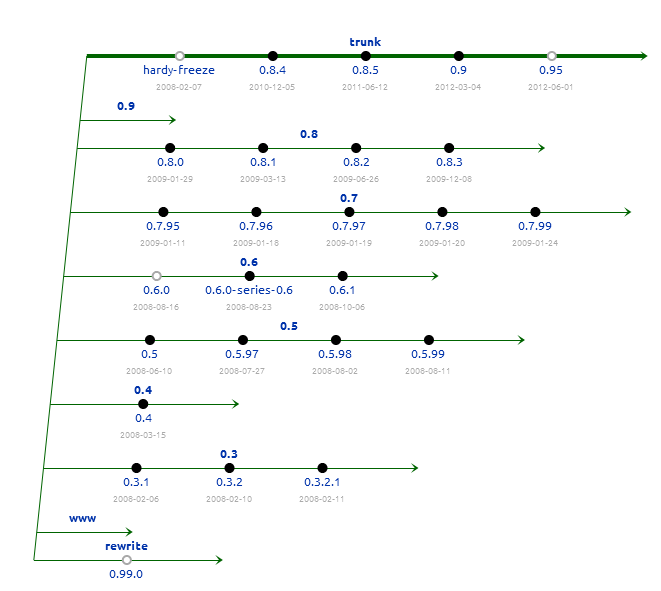
\includegraphics[width=1\linewidth]{tijdlijn}}
\caption{tijdlijn}
\label{tijdlijn}
\end{figure}

\cite{release}
\newpage % Begins the essay on a new page instead of on the same page as the table of contents



%------------------------------------------------
\subsection{Gnome-Do vs Launchy} % Sub-section
%------------------------------------------------
\subsubsection{Installatie}

\begin{tabularx}{1\textwidth}{|>{\setlength\hsize{1\hsize}\raggedright}X|>{\setlength\hsize{1\hsize}\raggedright}X|}
  \hline
Gnome-do &  Launchy\tabularnewline
\hline
  Goed geintegreerd en makkelijk te vinden in de softwaremap  & Niet standaard in de softwaremap. Installatie gebeurt van de bron  \tabularnewline
  \hline
\end{tabularx}





\subsubsection{Inteface}
\begin{tabularx}{1\textwidth}{|>{\setlength\hsize{1\hsize}\raggedright}X|>{\setlength\hsize{1\hsize}\raggedright}X|}
  \hline
Gnome-do &  Launchy\tabularnewline
\hline
  Aantrekkelijke interface die zich opent wanneer de Windowstoets en de spatie word ingedrukt. Onmiddellijk zoeken via toetsenbord, maar het woord wordt niet volledig weergegeven  & Makkelijk te bereiken via Windows toets. Laat het volledige woord zien dat ingegeven wordt.  \tabularnewline
  \hline
\end{tabularx}


\subsubsection{Plugins}
\begin{tabularx}{1\textwidth}{|>{\setlength\hsize{1\hsize}\raggedright}X|>{\setlength\hsize{1\hsize}\raggedright}X|}
  \hline
Gnome-do &  Launchy\tabularnewline
\hline
  Tal van plugins met verschillende functionaliteiten  & Minder plugins als Gnome-do  \tabularnewline
  \hline
\end{tabularx}

\subsubsection{Conclusie}
Gnome-do komt er beter uit dan Launchy. In geen enkel opzicht het is nodig over te schakelen van Gnome-do naar Launchy. Misschien als er in de toekomst meer plugins beschikbaar zijn voor Launchy, maar, dat is nu nog niet aan de orde. \cite{fosswire}

%----------------------------------------------------------------------------------------



\newpage % Begins the essay on a new page instead of on the same page as the table of contents




%----------------------------------------------------------------------------------------
\begin{BIJLAGE}
\newcommand{\HRule}{\rule{\linewidth}{0.5mm}} % Defines a new command for the horizontal lines, change thickness here
\center % Center everything on the page
\vspace*{\fill}
\HRule \\[0.4cm]
{ \huge \bfseries BIJLAGE}\\[0.4cm] % Title of your document
\HRule \\[1.5cm]
\vfill % Fill the rest of the page with whitespace
\end{titlepage}
%----------------------------------------------------------------------------------------



\newpage % Begins the essay on a new page instead of on the same page as the table of contents



%----------------------------------------------------------------------------------------

\section{Bijlage: Mailserver} 
Er zijn enkele stappen nodig om de mailserver te configeren. Deze stappen worden één voor één uitgelegd met eventuele printscreens.



\begin{figure}[H] % Example image
\center{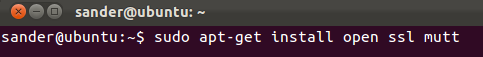
\includegraphics[width=0.5\linewidth]{1}}
\caption{Bijlage: Ingave in terminal}
\label{Bijlage: Ingave in terminal}
\end{figure}

\vspace{5 mm}

\begin{figure}[H] % Example image
\center{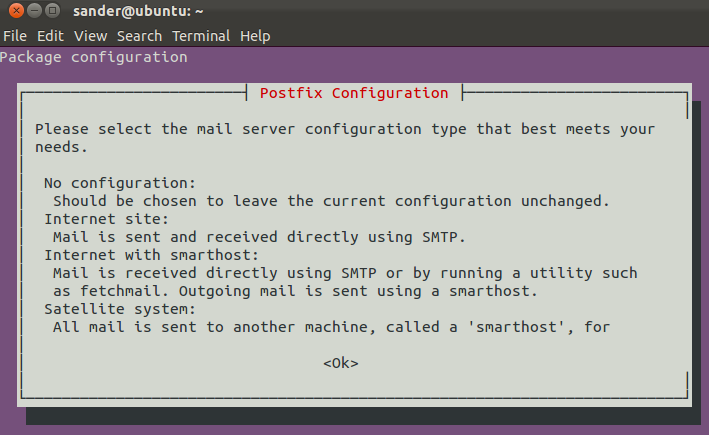
\includegraphics[width=0.5\linewidth]{mut3}}
\caption{Bijlage: Mailserver}
\label{Bijlage: Mailserver}
\end{figure}

\vspace{5 mm}

\begin{figure}[H] % Example image
\center{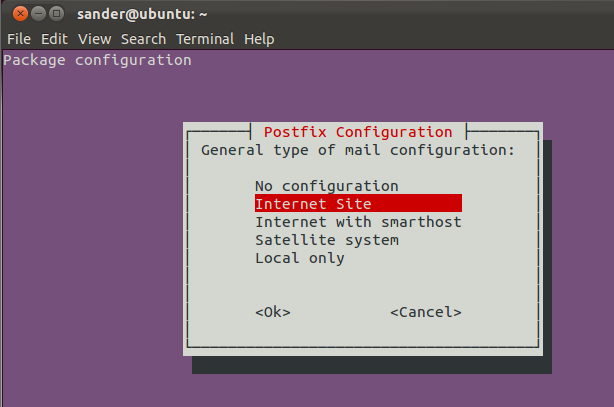
\includegraphics[width=0.5\linewidth]{mut4}}
\caption{Bijlage: Mailserver}
\label{Bijlage: Mailserver}
\end{figure}

\vspace{5 mm}

\begin{figure}[H] % Example image
\center{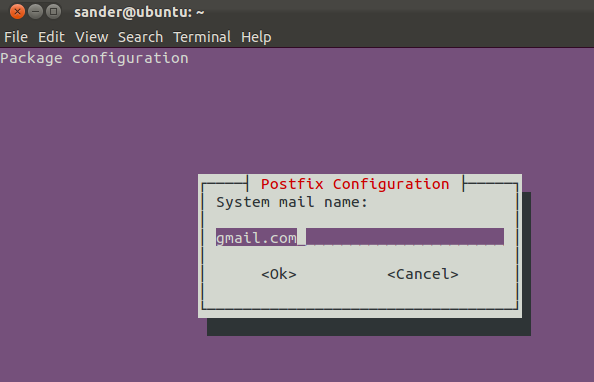
\includegraphics[width=0.5\linewidth]{mut5}}
\caption{Bijlage: Mailserver}
\label{Bijlage: Mailserver}
\end{figure}

\vspace{5 mm}

Nu de installatie voltooid is, moeten er enkel nog bepaalde gegevens bijgevoegd worden. In de map \etc bevindt zich een bestand .muttrc waarin aanpassingen dienen gedaan te worden. Volgende gegevens dienen onderaan het bestand bijgevoegd te worden:

\vspace{5 mm}

\begin{figure}[H] % Example image
\center{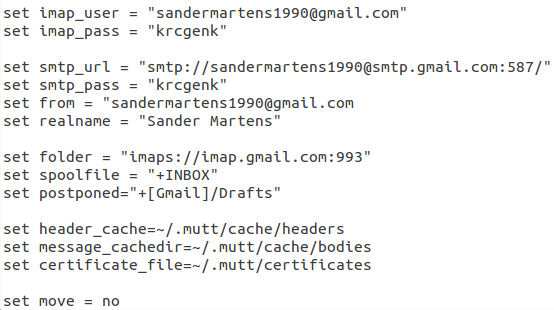
\includegraphics[width=0.5\linewidth]{mut6}}
\caption{Bijlage: gegevens mailserver}
\label{Bijlage: Gegevens mailserver}
\end{figure}
\end{Bijlage: Mailserver}
%----------------------------------------------------------------------------------------



\newpage % Begins the essay on a new page instead of on the same page as the table of contents



\section{Bijlage: Versiebeheer} \cite{git}

\setlength{\parindent}{0pt}Om git te configureren, dient onderstaande codes ingegeven te worden:
\begin{figure}[H] % Example image
\center{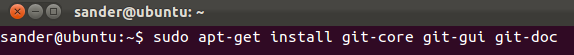
\includegraphics[width=0.5\linewidth]{git1}}
\caption{Bijlage: git1}
\label{Bijlage: git1}
\end{figure}

\vspace{5 mm}

\begin{figure}[H] % Example image
\center{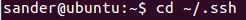
\includegraphics[width=0.5\linewidth]{git2}}
\caption{Bijlage: git2}
\label{Bijlage: git2}
\end{figure}

\vspace{5 mm}

\begin{figure}[H] % Example image
\center{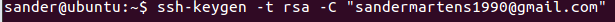
\includegraphics[width=0.5\linewidth]{git3}}
\caption{Bijlage: git3}
\label{Bijlage: git3}
\end{figure}

\vspace{5 mm}

\setlength{\parindent}{0pt}Na het ingeven van de vorige code wordt er gevraagd om een zin in te geven voor het wachtwoord. Dit is niet verplicht. Vervolgens dient er een account aangemaakt te worden op de website: https://github.com/ . Als dit gebeurd is, dient de SSH sleutel hier ingegeven te worden. De sleutel bevindt zich in de file met naam id\_rsa.pub . Eenmaal dit achter de rug, kunnen de volgende codes ingegeven worden.

\vspace{5 mm}

\begin{figure}[H] % Example image
\center{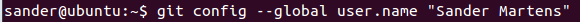
\includegraphics[width=0.5\linewidth]{git4}}
\caption{Bijlage: git4}
\label{Bijlage: git4}
\end{figure}

\vspace{5 mm}

\begin{figure}[H] % Example image
\center{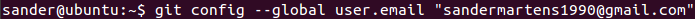
\includegraphics[width=0.5\linewidth]{git5}}
\caption{Bijlage: git5}
\label{Bijlage: git5}
\end{figure}
\end{Bijlage: Versiebeheer} 

\vspace{5 mm}

Vervolgens kan er een repository aangemaakt worden op de site. Dit is gewoon de stappen volgen en u bent klaar.

\newpage % Begins the essay on a new page instead of on the same page as the table of contents

\section{Bijlage: Bash-script}
zie bestand.

\vspace{5 mm}

referenties kunnen niet gemaakt worden om ongeldige reden.
%	BIBLIOGRAPHY
%----------------------------------------------------------------------------------------
\nocite{*}
\bibliographystyle{plain}
\bibliography{referentie}
%----------------------------------------------------------------------------------------

\end{document}
